\documentclass[../main.tex]{subfiles}
\ifSubfilesClassLoaded{\setcounter{chapter}{7}}{}
\begin{document}

\chapter{Regresi Linear dan Metrik RMSE/MAE}

\begin{subcpmk}
  \item \textbf{Sub-CPMK-P6:} Melatih regresi linear (atau Ridge); melaporkan RMSE/MAE pada data uji; membandingkan dengan baseline (RPS Mg.\ 7).
\end{subcpmk}

\SesiRPS{7}{P6}{$\sim$170 menit}{CPMK-P3}

\noindent Regresi linear tetap berguna sebagai \textbf{model dasar} yang cepat dan mudah diinterpretasikan. Membandingkan RMSE/MAE dengan baseline rata-rata menjawab: ``apakah fitur yang dipakai benar-benar menurunkan error prediksi?''

\section{Kemampuan akhir sesi}

Melatih regresi pada data uji terpisah; melaporkan RMSE dan MAE dalam satuan target; menjelaskan perbedaan sensitivitas kedua metrik terhadap outlier error; memakai \texttt{Pipeline} bila skala fitur berbeda jauh.

Metrik pada data uji mencerminkan kinerja \textit{out-of-sample}, lebih realistis daripada residual hanya pada data latih.

\section{Teori}

\begin{konsep}
Regresi memprediksi target kontinu. RMSE dan MAE mengukur error dalam satuan target. Baseline rata-rata memberi acuan minimal: model harus mengalahkan baseline yang masuk akal.
\end{konsep}

\begin{catatan}
Gunakan \path{sklearn.metrics.root_mean_squared_error} (versi baru) atau \path{mean_squared_error(..., squared=False)} sesuai versi paket terpasang.
\end{catatan}

Ridge (\textit{regularisasi} L2) membantu ketika fitur berkolinear atau dimensi tinggi; koefisien menjadi lebih stabil dibanding Ordinary Least Squares murni. \texttt{Pipeline} dengan \texttt{StandardScaler} sering dipasangkan dengan Ridge/SVM untuk konsistensi skala.

\begin{figure}[htbp]
\centering
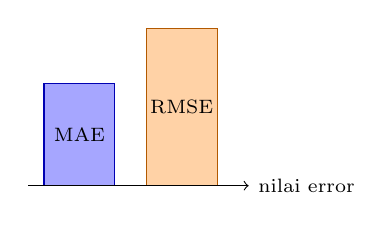
\begin{tikzpicture}[x=1cm,y=1cm]
  \draw[fill=blue!35, draw=blue!70!black] (0,0) rectangle (0.9,1.3)
    node[midway, font=\scriptsize, align=center] {MAE};
  \draw[fill=orange!35, draw=orange!70!black] (1.3,0) rectangle (2.2,2.0)
    node[midway, font=\scriptsize, align=center] {RMSE};
  \draw[->] (-0.2,0) -- (2.6,0) node[right, font=\scriptsize] {nilai error};
\end{tikzpicture}
\caption{Ilustrasi konseptual: pada outlier besar, RMSE cenderung lebih tinggi dari MAE karena kuadrat error; pilih metrik sesuai sensitivitas bisnis terhadap error ekstrem.}
\end{figure}


\begin{table}[htbp]
\centering
\caption{LinearRegression vs Ridge (intuisi pemilihan).}
\label{tab:linear-ridge}
\begin{tabular}{@{}p{3.6cm}p{9.1cm}@{}}
\toprule
\textbf{Model} & \textbf{Kapan pertama kali dicoba} \\
\midrule
\texttt{LinearRegression} & Baseline interpretatif; hubungan hampir linear. \\
\texttt{Ridge} & Banyak fitur berkorelasi; perlu stabilisasi koefisien. \\
\bottomrule
\end{tabular}
\end{table}

\section{Contoh kode}

Dataset \path{load_diabetes} dari \texttt{sklearn.datasets} adalah contoh regresi klasik berdimensi tetap; sesuaikan \path{test_size} dan \path{random_state} dengan kebijakan lab.

\MulaiPenjelasanKode \texttt{LinearRegression} meminimalkan MSE ordinari; metrik \texttt{MAE} dan \texttt{RMSE} mengukur error pada \textbf{data uji} setelah model di-\texttt{fit} pada train. \SelesaiPenjelasanKode

\begin{lstlisting}[caption=Dataset diabetes dan split]
from sklearn.datasets import load_diabetes
from sklearn.model_selection import train_test_split
from sklearn.linear_model import LinearRegression
from sklearn.metrics import mean_absolute_error, root_mean_squared_error

X, y = load_diabetes(return_X_y=True)  # X: 10 fitur terstandar; y: progresi penyakit (target kontinu)
X_train, X_test, y_train, y_test = train_test_split(
    X, y, test_size=0.2, random_state=42  # regresi: stratify tidak dipakai (bukan klasifikasi)
)
model = LinearRegression()  # model linier tanpa penalti L2 eksplisit (OLS dengan regularisasi minimal sklearn)
model.fit(X_train, y_train)  # estimasi koefisien dari train
pred = model.predict(X_test)  # nilai kontinu prediksi per baris test
print("MAE", mean_absolute_error(y_test, pred))  # rata-rata |error|
print("RMSE", root_mean_squared_error(y_test, pred))  # akar MSE (sensitif outlier error besar)
\end{lstlisting}

\MulaiPenjelasanKode Baseline memprediksi konstanta = rata-rata target train; RMSE baseline menunjukkan apakah model linier memberi peningkatan bermakna. \SelesaiPenjelasanKode

\begin{lstlisting}[caption=Baseline prediksi rata-rata]
import numpy as np
base_pred = np.full_like(y_test, fill_value=y_train.mean(), dtype=float)  # vektor sama panjang y_test, isi mean train
print("RMSE baseline", root_mean_squared_error(y_test, base_pred))
\end{lstlisting}

\MulaiPenjelasanKode \path{Ridge(alpha=...)} menambah penalti L2 pada koefisien; \path{StandardScaler} di pipeline menstandarkan fitur agar besaran penalti seimbang antar fitur. \SelesaiPenjelasanKode

\begin{lstlisting}[caption=Pipeline dengan scaling (disarankan)]
from sklearn.pipeline import Pipeline
from sklearn.preprocessing import StandardScaler
from sklearn.linear_model import Ridge

pipe = Pipeline([
    ("scale", StandardScaler()),  # langkah 1: z-score fit dari train, transform train+test
    ("reg", Ridge(alpha=1.0)),  # langkah 2: regresi ridge; alpha: kuat penalti L2
])
pipe.fit(X_train, y_train)  # fit scaler dan regresor secara berurutan pada train
pred2 = pipe.predict(X_test)  # prediksi test dengan parameter hasil train
\end{lstlisting}

\section{Referensi}

\begin{itemize}[leftmargin=*]
  \item ISLR (teori). \url{https://www.statlearning.com/}
  \item Python Data Science Handbook. \url{https://jakevdp.github.io/PythonDataScienceHandbook/}
\end{itemize}

\begin{asesmen}
\textbf{Tugas modul:} RMSE/MAE pada test + perbandingan baseline; gunakan Pipeline jika ada fitur numerik skala berbeda.
\end{asesmen}

\begin{rangkuman}
Minggu 7 menghubungkan model regresi dengan interpretasi error pada data uji.

\textbf{Kata kunci:} LinearRegression, Ridge, RMSE, MAE, baseline
\end{rangkuman}

\end{document}
